%%%%%%%%%%%%%%%%%%%%%%%%%%%%%%%%%%%%%%%%%%%%%%%%%%%%%%%%%%%%%%%%%%%%%%%%%%%%%%%%%%%%%%%%%%%%%%%%%%%%%%%%%%%%%%%%%%%%%%%%%%%%%%%%%%%%%%%%%
\section{Channel selection}\label{sec:esnr_chansel}
The goal of a \emph{channel selection} algorithm is to quickly choose the best operating frequency for a pair of nodes to communicate. In this section, I define the ``best'' channel to be the channel that provides the highest throughput in the absence of interferers.

%%%%%%%%%%%%%%%%%%%%%%%%%%%%%%%%%%%%%%%%%%%%%%%%%%%%%%%%%%%%%%%%%%%%%%%%%%%%%%%%%%%%%%%%%%%%%%%%%%%%%%%%%%%%%%%%%%%%%%%%%%%%%%%%%%%%%%%%%
\subsection{Characterization of 802.11 channels}
To start my investigation of channel selection algorithms, I first measured how the operating frequency affects 802.11n links in practice.

\subsubsection{Measurements}
\label{sec:chan_sel_data}
The \term{iwl5300} devices in the testbed can operate on 35 channels, each 20\MHz wide, defined by IEEE 802.11 standard. Of these 35 channels, 11 overlap in the 83-\MHz wide unlicensed 2.4\GHz band, and the remaining 24 non-overlapping channels are spread across three non-contiguous bands between 5.170\GHz and 5.835\GHz.

For the results presented in this section, I measured the physical RF channel (using both RSS and CSI) and actual packet delivery using each of the 24 IEEE 802.11n modulation and coding schemes (MCS~0--MCS~23) that use  1-, 2-, or 3-streams. I measured these data for all links between 24 testbed nodes at UW\@. Each sender transmits packets with random payloads, sending a total of 2400 packets by interleaving 100 packets from each of the 1-, 2-, or 3-stream 802.11n rates. Each receiver uses 3 antennas for spatial diversity and/or spatial multiplexing. From these data, we can compute the expected throughput $T$ for a particular link $\ell$ and MCS~$m$ as
\begin{equation}
	\label{eq:prr_throughput}
	T(\ell,m) = \frac{P(\ell,m)}{100} \cdot B(m),
\end{equation}
where $P(\ell,m)$ is the number of packets delivered on link $\ell$ at MCS~$m$ and $B(m)$ is the raw bitrate of MCS~$m$.

\subsubsection{Impact of operating channel}
To understand whether the choice of operating channel matters in practice, I measured the throughput for each link as a function of 802.11 channel. Since there is considerable Wi-Fi interference in our building on the entire 2.4\GHz band and on many of the 5\GHz channels, I use a subset of data taken on the 11 channels in the 5\GHz band that the testbed nodes can use and are not shared with a UW CSE or nearby UW access point.

\begin{figure}[tp]
	\centering
	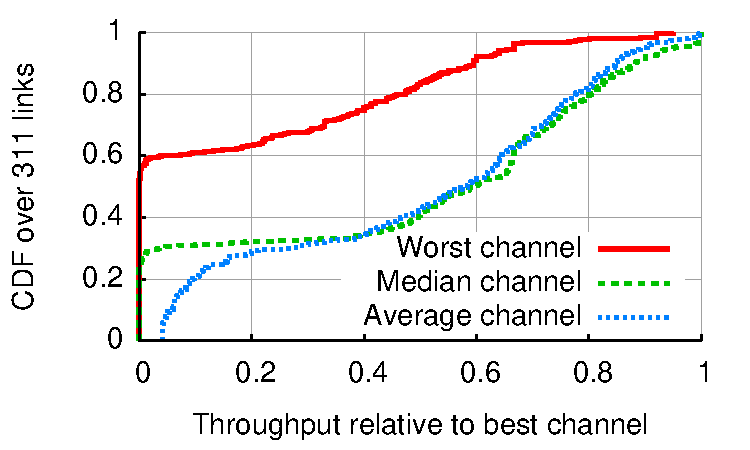
\includegraphics[width=0.6\textwidth]{figures/esnr/rel_diff.pdf}
	\caption{\label{fig:rel_diff}The relative difference in throughput over 802.11n channels.}
\end{figure}

\begin{figure}[tp]
	\centering
	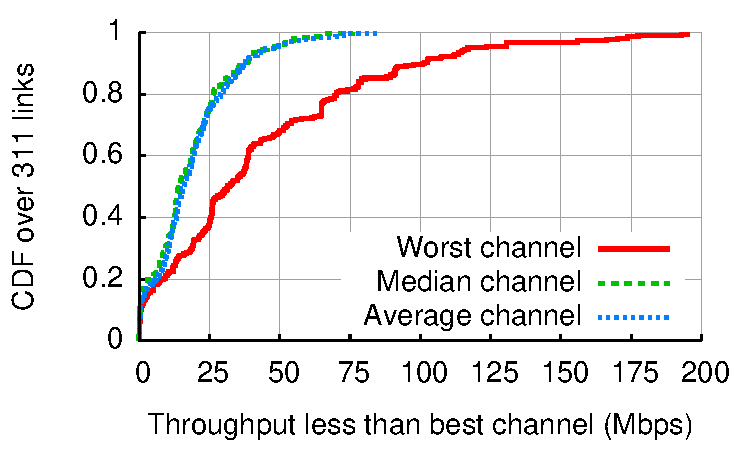
\includegraphics[width=0.6\textwidth]{figures/esnr/tpt_diff.pdf}
	\caption{\label{fig:tpt_diff}The absolute difference in throughput over 802.11n channels.}
\end{figure}

\figref{fig:rel_diff} and \figref{fig:tpt_diff} show how the throughput of the worst, median, and average channels compares to the best channel (with the highest throughput) for these links. \figref{fig:rel_diff} shows the relative throughput as a fraction of the throughput of the best channel, and \figref{fig:tpt_diff} shows the absolute difference between channels in Mbps. These figures demonstrate that the choice of channel can dramatically impact performance. The worst channel delivers no packets for more than half of the links, and offers less than half of the best throughput for more than 80\% of the links. In absolute terms, this difference can be quite large: the worst channel is a median 50\Mbps worse than the best channel, and for a few links the difference is more than 100\Mbps. For these links, some channel will deliver no packets at all, while another delivers packets at nearly the maximum bitrate. An unlucky choice of channel can cripple performance and result in little to no throughput.

The median and average channels perform about equivalently in our testbed, and even these are significantly worse. These channels yield less than half the optimal throughput for 40\% of the links and for only 20\% of links do these come within 80\% of the best throughput. These figures show that for very few links do most channels perform about the same, and the median or average channel is 10--25\Mbps worse than the best channel for most links, and the gap is larger than 25\Mbps for 20\% of links.

\subsubsection{Conclusion}
From these results, I conclude that a strategy that picks a fixed channel or a random channel will perform significantly worse than a strategy that can identify channels that are likely to offer good performance. Having motivated the need for an accurate channel selection algorithm, I present and evaluate different channel selection strategies in the rest of this section.

%%%%%%%%%%%%%%%%%%%%%%%%%%%%%%%%%%%%%%%%%%%%%%%%%%%%%%%%%%%%%%%%%%%%%%%%%%%%%%%%%%%%%%%%%%%%%%%%%%%%%%%%%%%%%%%%%%%%%%%%%%%%%%%%%%%%%%%%%
\subsection{Channel selection algorithms}
\algref{alg:chan_sel_basic} is a template for a channel selection algorithm. It takes as input a list of channels to evaluate $C$, and a sender $s$ and receiver $r$ that together define a link. The two nodes hop across channels, using the \fcall{PredictChannelThroughput} function to evaluate the performance of the link on each. The algorithm tracks the best performing channel, labeled $c_{\max}$ and returns that value. (\fcall{ChannelSelection} can also return $\emptyset$ if all channels have zero predicted throughput, but we only consider links that can communicate on at least 1 channel.) Using this template, different channel selection algorithms can be instantiated by providing different implementations of \fcall{PredictChannelThroughput}.

%%%%%%%%%%%%%%%%%%%%%%%%%%%%%%%%%%%%%%%%%%%%%%%%
\begin{algorithm}[htp]
\caption{\label{alg:chan_sel_basic}\fcall{ChannelSelection($C, s, r$)}}
\begin{algorithmic}
\STATE $t_{\max}\gets 0\Mbps$
\STATE $c_{\max} \gets \emptyset$
\FORALL{$c \in C$}
\STATE Both $s$ and $r$ switch to channel $c$
\STATE $t \gets \fcall{PredictChannelThroughput($c, s, r$)}$
\IF{$t > t_{\max}$}
	\STATE $t_{\max} \gets t$
	\STATE $c_{\max} \gets c$
\ENDIF
\RETURN $c_{\max}$
\ENDFOR
\end{algorithmic}
\end{algorithm}
%%%%%%%%%%%%%%%%%%%%%%%%%%%%%%%%%%%%%%%%%%%%%%%%

I consider three different channel selection algorithms in this section. The first is \fcall{ChannelSelectionOPT}, an oracular channel selection algorithm that chooses the optimal channel. For implementation purposes, I instantiate \fcall{ChannelSelectionOPT} by \algref{alg:chan_sel_probe} (\fcall{ProbeChannelThroughput}), which probes all MCSes with MTU-sized packets to determine packet delivery and predicts throughput according to \eqref{eq:prr_throughput}.

%%%%%%%%%%%%%%%%%%%%%%%%%%%%%%%%%%%%%%%%%%%%%%%%
\begin{algorithm}[tp]
\caption{\label{alg:chan_sel_probe}\fcall{ProbeChannelThroughput($c, s, r$)}}
\begin{algorithmic}
\STATE $p_0,p_1,\dots,p_{23} \gets 0$
\STATE $N \gets \text{number of probes at each MCS}$
\FOR{$i = 1 \dots N$}
\FOR{$m = 0 \dots 23$}
\STATE $s$ sends one MTU-sized packet at MCS~$m$
\IF{$s$ receives an ACK from $r$}
\STATE $p_m \gets p_m + 1$
\ENDIF
\ENDFOR
\ENDFOR
\STATE $t_{\max}\gets \max \{p_m/N \cdot M(m)\} \text{ over all } m$ \hfill \COMMENT{\eqref{eq:prr_throughput}}
\RETURN $t_{\max}$
\end{algorithmic}
\end{algorithm}
%%%%%%%%%%%%%%%%%%%%%%%%%%%%%%%%%%%%%%%%%%%%%%%%
%%%%%%%%%%%%%%%%%%%%%%%%%%%%%%%%%%%%%%%%%%%%%%%%
\begin{algorithm}[tp]
\caption{\label{alg:chan_sel_rss}\fcall{PredictChannelThroughputRSS($c, s, r$)}}
\begin{algorithmic}
\STATE $s$ sends one packet with 0-byte payload at MCS~0
\STATE $r$ computes the RSS $R$ and returns it along with the ACK
\IF{$s$ receives an ACK from $r$}
\RETURN \fcall{RSSToThroughput($R$)}, $R$ \hfill \COMMENT{the RSS $R$ is used to break ties}
\ELSE
\RETURN 0
\ENDIF
\end{algorithmic}
\end{algorithm}
%%%%%%%%%%%%%%%%%%%%%%%%%%%%%%%%%%%%%%%%%%%%%%%%
%%%%%%%%%%%%%%%%%%%%%%%%%%%%%%%%%%%%%%%%%%%%%%%%
\begin{algorithm}[tp]
\caption{\label{alg:chan_sel_esnr}\fcall{PredictChannelThroughputESNR($c, s, r$)}}
\begin{algorithmic}
\FOR{$m \in \{16, 8, 0\}$}
\STATE $s$ sends one packet with 0-byte payload at MCS~$m$
\STATE $r$ computes the Effective SNR values $\rho_\text{eff}$ and returns them along with the ACK
\IF{$s$ receives an ACK from $r$}
	\RETURN \fcall{ESNRToThroughput}($\rho_\text{eff}$), $\rho_\text{eff}$ \hfill \COMMENT{$\rho_\text{eff}$ is used to break ties}
\ENDIF
\ENDFOR
\RETURN 0
\end{algorithmic}
\end{algorithm}
%%%%%%%%%%%%%%%%%%%%%%%%%%%%%%%%%%%%%%%%%%%%%%%%

The second algorithm chooses the channel based on RSS, presented in \algref{alg:chan_sel_rss}. In this case, the sender only needs to send a single probe packet (with no payload) in order to measure the RSS on the channel. Since \fcall{RSSToThroughput} is monotonically increasing in RSS, this algorithm is equivalent to selecting the channel with the maximum RSS\@.

The third algorithm chooses the channel based on the Effective SNR, presented in \algref{alg:chan_sel_esnr}. Here, the sender sends probes (with no payload) with decreasing numbers of spatial streams to enable the receiver to collect a maximal CSI measurement. The receiver then sends the computed Effective SNR values back to the sender, which uses them to predict the best rate.

I evaluate these three algorithms in the next section.

%%%%%%%%%%%%%%%%%%%%%%%%%%%%%%%%%%%%%%%%%%%%%%%%%%%%%%%%%%%%%%%%%%%%%%%%%%%%%%%%%%%%%%%%%%%%%%%%%%%%%%%%%%%%%%%%%%%%%%%%%%%%%%%%%%%%%%%%%
\subsection{Evaluation}
To evaluate the three channel selection algorithms I presented in the previous section, I use the measurements described in \secref{sec:chan_sel_data}. In the 24-node UW testbed, there are $24*23=552$ ordered pairs of nodes that can form unidirectional links. To consider only non-trivial cases of channel selection, I restrict my analysis in this section to the 201 of these 552 links can deliver packets on at least 3 different channels.

%%%%%%%%%%%%%%%%%%%%%%%%%%%%%%%%%%%%%%
\subsubsection{Channel selection accuracy}
\figref{fig:chan_sel_ratio_opt} shows the performance relative to the optimal algorithm when using Effective SNR and RSS to choose between channels. I plot the complementary CDF of the links, so that each $(x,y)$ point in the graph shows the fraction of links $y$ that achieved performance at least a fraction $x$ of the optimal algorithm. The line for an accurate algorithm would be located in the upper right corner of the graph: most links would achieve most of the best possible throughput. This figure shows that both algorithms perform well, though choosing channel based on Effective SNR is more accurate than based on RSS\@.

\begin{figure}[htp]
	\centering
	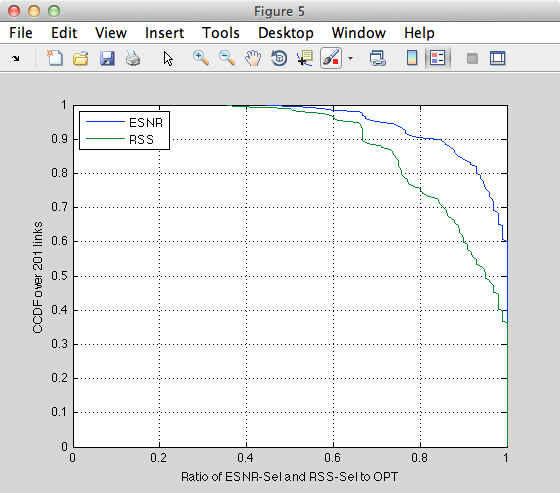
\includegraphics[width=0.6\textwidth]{figures/esnr/chan_sel_ratio_opt.png}
	\caption{\label{fig:chan_sel_ratio_opt}Channel selection algorithm performance relative to an optimal algorithm.}
\end{figure}

In this figure, Effective SNR chooses an optimal channel for 121 links (60\%), whereas RSS is optimal for only 73 links (36\%). The Effective SNR-based algorithm is within 90\% of optimal for 161 links (84\%), 80\% for 181 links (90\%), and 70\% for 191 links (95\%). In contrast, maximizing RSS only gets within 90\% of optimal for 123 links (61\%).

\begin{figure}[htp]
	\centering
	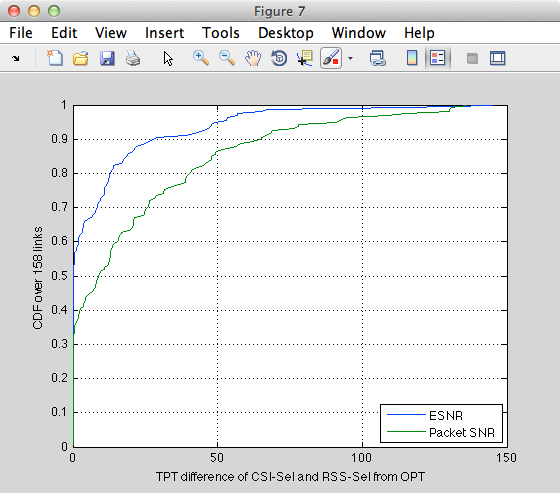
\includegraphics[width=0.6\textwidth]{figures/esnr/chan_sel_delta_opt.png}
	\caption{\label{fig:chan_sel_delta_opt}Channel selection algorithm performance loss from optimal algorithm.}
\end{figure}

Next, I compare the absolute performance loss of the channel selection algorithms in \figref{fig:chan_sel_delta_opt}. Here, each $(x,y)$ point represents the fraction of links $y$ that choose a channel within $y$\Mbps of the best channel with a particular algorithm. The area over the curves represents the performance lost by each algorithm; an accurate algorithm would be in the top left corner, losing little throughput for only a few links. This area is 2.9$\times$ larger for the RSS-based selection algorithm, showing that Effective SNR is significantly more accurate. This difference translates to about 10\Mbps more per link when selecting channels via the Effective SNR\@.

\begin{figure}[htp]
	\centering
	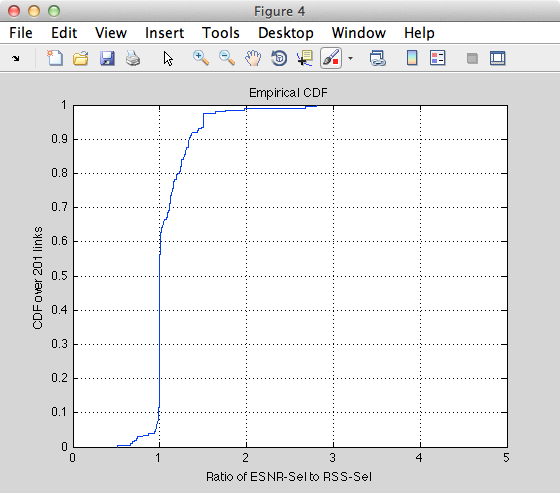
\includegraphics[width=0.6\textwidth]{figures/esnr/chan_sel_ratio.png}
	\caption{\label{fig:chan_sel_ratio}Channel selection performance with Effective SNR relative to RSS\@.}
\end{figure}

Finally, I examine the head-to-head performance of selecting channels via Effective SNR or RSS in \figref{fig:chan_sel_ratio}. For each link, I plot the ratio of the performance of the channel picked with the Effective SNR strategy to that of the channel chosen by maximizing RSS\@. If the two channels perform equally, the ratio will be 1; if the Effective SNR strategy chose a better channel the ratio will be larger. The algorithms choose channels with equal performance for 90 (45\%) of the 201 links, while the Effective SNR-based algorithm chooses a better channel for 88 (44\%) links and the RSS-based algorithm for the remaining 23 (11\%). Additionally, the gains from Effective SNR are much larger than its losses: the RSS strategy chooses a channel that performs 20\% better than the Effective SNR-selected channel for only 6/23 (26\%) links its channel is better, while Effective SNR chooses a 20\% better channel for 41/88 (47\%) of cases. In other words, the Effective SNR channel selection algorithm is more likely to pick a better channel by a factor of about 4 (88/23), and this difference is more likely to be significant by a factor of about 2 (47\%/26\%).

In conclusion, these results shows that both Effective SNR- and RSS-based channel selection strategies perform well for 3-stream IEEE 802.11n links. However, the Effective SNR channel selection strategy is significantly more accurate: it chooses an optimal channel for 66\% more links, it offers about 10\Mbps more per link when selecting suboptimal channels, and it is more likely to choose a better channel by a factor of 4.

%%%%%%%%%%%%%%%%%%%%%%%%%%%%%%%%%%%%%%
\subsubsection{Channel discrimination}
\begin{itemize}
\item with multiple antennas, all channels within a band are roughly equivalent RSS\@. in 5\GHz, can see variability plausibly attributable to the actual antenna response.

\begin{figure}[htp]
	\centering
	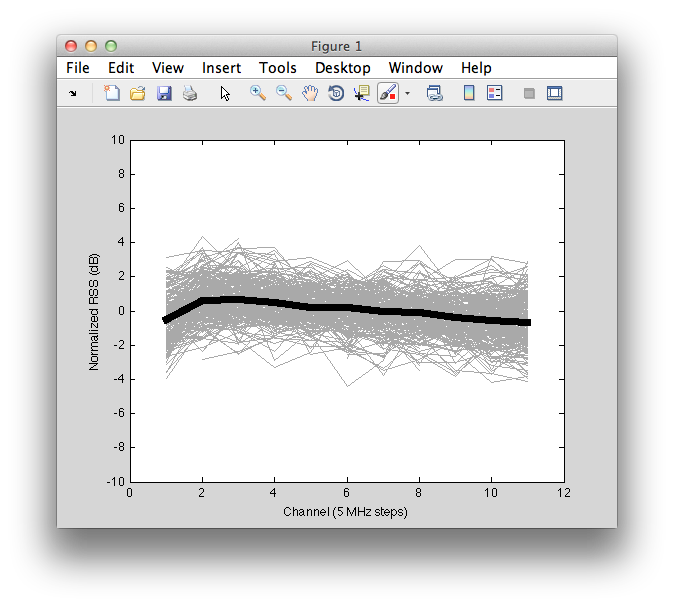
\includegraphics[width=\textwidth]{figures/esnr/rssi_vs_freq_24.png}
	\caption{\label{fig:rssi_vs_freq_24}RSS versus 2.4\GHz channel for 249 links. Solid line shows the median for each channel.}
\end{figure}
\begin{figure}[htp]
	\centering
	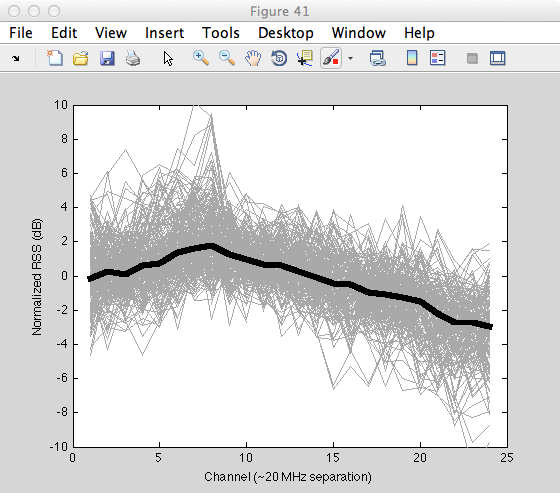
\includegraphics[width=\textwidth]{figures/esnr/rssi_vs_freq_5.png}
	\caption{\label{fig:rssi_vs_freq_5}RSS versus 5\GHz channel for 163 links. Solid line shows the median for each channel.}
\end{figure}
\begin{figure}[htp]
	\centering
	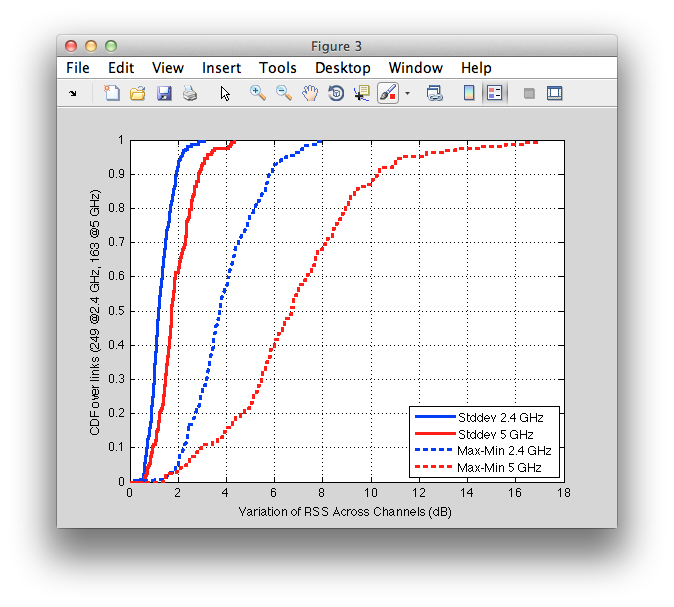
\includegraphics[width=\textwidth]{figures/esnr/rssi_freq_dev.png}
	\caption{\label{fig:rssi_freq_dev}Standard deviation and max-min spread of RSS across channels within the same band.}
\end{figure}

\item \figref{fig:rel_diff_draws} shows that, depending on how close to optimal you want to be, need to look at 5, 10, or 15 of the 24 channels in 5\GHz band. If we can evaluate the rate offered by a channel quickly, we can look at more channels in the same amount of time to pick the best rate.
\end{itemize}

\begin{figure}[htp]
	\centering
	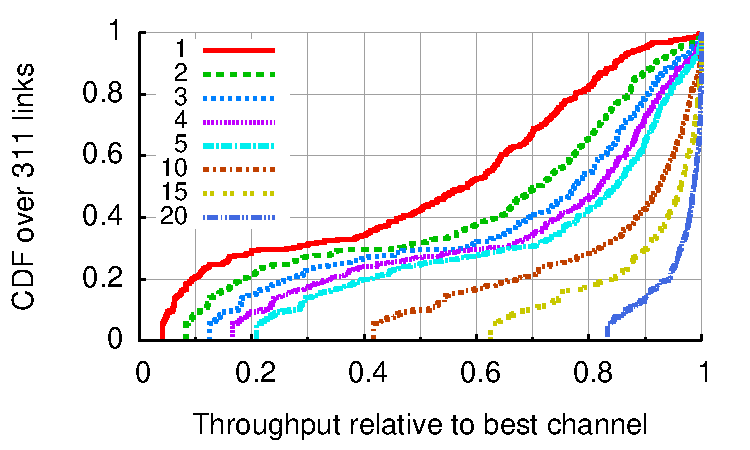
\includegraphics[width=0.6\textwidth]{figures/esnr/rel_diff_draws.pdf}
	\caption{\label{fig:rel_diff_draws}The expected rate after choosing the best of $k$ 802.11n channels.}
\end{figure}

%%%%%%%%%%%%%%%%%%%%%%%%%%%%%%%%%%%%%%%%%%%%%%%%%%%%%%%%%%%%%%%%%%%%%%%%%%%%%%%%%%%%%%%%%%%%%%%%%%%%%%%%%%%%%%%%%%%%%%%%%%%%%%%%%%%%%%%%%
\subsection{Further Evaluations?}
\heading{Performance.}  given time to hop $\mathcal{O}$(1\ms), time to execute a CSI probe $\mathcal{O}$(500\us), and time to execute a rate probe (unknown), how many channels can we look at in $T$ time? Reference \figref{fig:rel_diff_draws} to see what fraction of optimal this enables.

\heading{Completion Time.} The difference between the Effective SNR and the SNR is a proxy for how ``good'' a channel is, based on how flat it is. Given that RSS is similar across channels, the flattest channel will likely offer the best rate. Can we use this to detect a good channel and stop looking early?